\documentclass[12pt]{article}

\usepackage{times}
\topmargin 0.0cm
\oddsidemargin 0.2cm
\textwidth 16cm
\textheight 21cm
\footskip 1.0cm

\usepackage{indentfirst}
\usepackage{graphicx}
\usepackage[utf8]{inputenc}
\usepackage[round]{natbib}
\bibliographystyle{abbrvnat} % ou usar: rusnat




% \citet{Anderson2011} para produzir Anderson et al. (2011)
% \citep{Anderson2011} para produzir (Anderson et al. 2011)



\usepackage{lineno,xcolor} 	% See \linenumbers at the top of content.tex
% Include your paper's title here
%\usepackage[backend=biber]{biblatex}
%\bibliography{library}

\title{My Manuscript Title}

%       Comando      Declaração
%  Bold \textbf{...} {\bfseries...}
%Máquina de escrever \texttt{...} {\ttfamily...}
%Itálico \textit{...} {\itshape...}

\author
{John Smith,$^{1\ast}$ Jane Doe,$^{1}$ Joe Scientist$^{2}$\\
\\
\normalsize{$^{1}$Department of Chemistry, University of Wherever,}\\
\normalsize{An Unknown Address, Wherever, ST 00000, USA}\\
\normalsize{$^{2}$Another Unknown Address, Palookaville, ST 99999, USA}\\
\\
\normalsize{$^\ast$To whom correspondence should be addressed; E-mail:  jsmith@wherever.edu.}
}

% Include the date command, but leave its argument blank.

\date{}



%%%%%%%%%%%%%%%%% END OF PREAMBLE %%%%%%%%%%%%%%%%



\begin{document}
%\maketitle % Insert title

% NOTE: Comment out the lines below to remove line numbers
  % Running line numbers:
  \linenumbers
  \setlength\linenumbersep{15pt}
  \renewcommand\linenumberfont{\normalfont\footnotesize\sffamily\color{gray}}
  %\pagewiselinenumbers % Same, but that reset on every page:
  \modulolinenumbers[1] % Number only every line. Change for fewer.

% Double-space the manuscript.

\baselineskip24pt

% Make the title.

\maketitle

% Place your abstract within the special {sciabstract} environment.
% ABSTRACT
\section*{Abstract}

This document presents a number of hints about how to set up your \texttt{scifile.tex}.
That you can use to set up the \LaTeX\ source \texttt{\{sciabstract\}} environment used to set up the abstract you

% INTRODUCTION

\section*{Introduction}

In this file, we present some tips and sample mark-up to assure your
\LaTeX\ file of the smoothest possible journey from review manuscript
to published {\it Science\/} paper.  We focus here particularly on
issues related to style files, citation, and math, tables, and
figures, as those tend to be the biggest sticking points.  Please use
the source file for this document, \texttt{scifile.tex}, as a template
for your manuscript, cutting and pasting your content into the file at
the appropriate places.


Citando 2 aqui \citet{Shipley2009}


{\it Science\/}'s publication workflow relies on Microsoft Word.  To translate % cosmcosmosmcsopcmSP~CÇOMopslm
\LaTeX\ files into Word, we use an intermediate MS-DOS routine that converts % LICNAÇLKCNALIDVNÇOAIL.N
the \TeX\ source into HTML\@.  Theroutine is generally robust, but it works best if the source document is clean \LaTeX\ without a significant freight of local macros or \texttt{.sty} files.  Use of the source file \texttt{scifile.tex} as a template, and calling {\it only\/} the \texttt{.sty} and \texttt{.bst} files specifically mentioned here, will generate a manuscript that should be eminently reviewable, and yet will allow your paper to proceed quickly into our production flow upon acceptance .

% MATERIAL AND METHODS

\section*{Material and Methods}

In this file, we present some tips and sample mark-up to assure your % lçkjçlskfjdglkfjsgçlkfs.m,g 
\LaTeX\ file of the smoothest possible journey from review manuscript %.nçlkfnsçofdlkgnbçodliknb~lg;l
to published {\it Science\/} paper.  We focus here particularly on
issues related to style files, citation, and math, tables, and
figures, as those tend to be the biggest sticking points.  Please use
the source file for this document, \texttt{scifile.tex}, as a template
for your manuscript, cutting and pasting your content into the file at
the appropriate places. 
% RESULTS

\section*{Results}

In this file, we present some tips and sample mark-up to assure your
\LaTeX\ file of the smoothest possible journey from review manuscript
to published {\it Science\/} paper.  We focus here particularly on
issues related to style files, citation, and math, tables, and
figures, as those tend to be the biggest sticking points.  Please use
the source file for this document, \texttt{scifile.tex}, as a template
for your manuscript, cutting and pasting your content into the file at
the appropriate places. 

\begin{table}[h]
	\centering
	\caption{A minha tabela ficou muito mais bonita do que a do template.} 
	\label{tab1}
	\begin{tabular}{ccc}
		\hline \rule[-2ex]{0pt}{5.5ex} Espécies & Abundância & Frequência \\ 
		\hline \rule[-2ex]{0pt}{5.5ex} \textbf{Banana} & 1878 & 45 \\ 
		\hline \rule[-2ex]{0pt}{5.5ex} \textit{Maça} & 456 & \textbf{34} \\ 
		\hline \rule[-2ex]{0pt}{5.5ex} Uva & 345 & 57 \\ 
		\hline \rule[-2ex]{0pt}{5.5ex} Jaca & 23 & 10 \\ 
		\hline \rule[-2ex]{0pt}{5.5ex} Jaca & 23 & 10 \\ 
		\hline \rule[-2ex]{0pt}{5.5ex} Jaca & 23 & 10 \\ 
		\hline \rule[-2ex]{0pt}{5.5ex} Jaca & 23 & 10 \\ 
		\hline \rule[-2ex]{0pt}{5.5ex} Jaca & 23 & 10 \\ 
		\hline 
	\end{tabular}
\end{table}

\input{sections/04_discussion}
% CONCLUSION

\section*{Conclusion}

In this file, we present some tips and sample mark-up to assure your
\LaTeX\ file of the smoothest possible journey from review manuscript
to published {\it Science\/} paper.  We focus here particularly on
issues related to style files, citation, and math, tables, and
figures, as those tend to be the biggest sticking points.  Please use
the source file for this document, \texttt{scifile.tex}, as a template
for your manuscript, cutting and pasting your content into the file at
the appropriate places. 


\section*{Ackownlegment}

\newpage
% \section*{References}
\bibliography{bibliography/library}

%\printbibliography

\newpage
\section*{Tables}
% \input{tables/sample_table.tex}



\newpage
\section*{Figures}

\begin{figure}[h]
	\centering % para centralizarmos a figura
	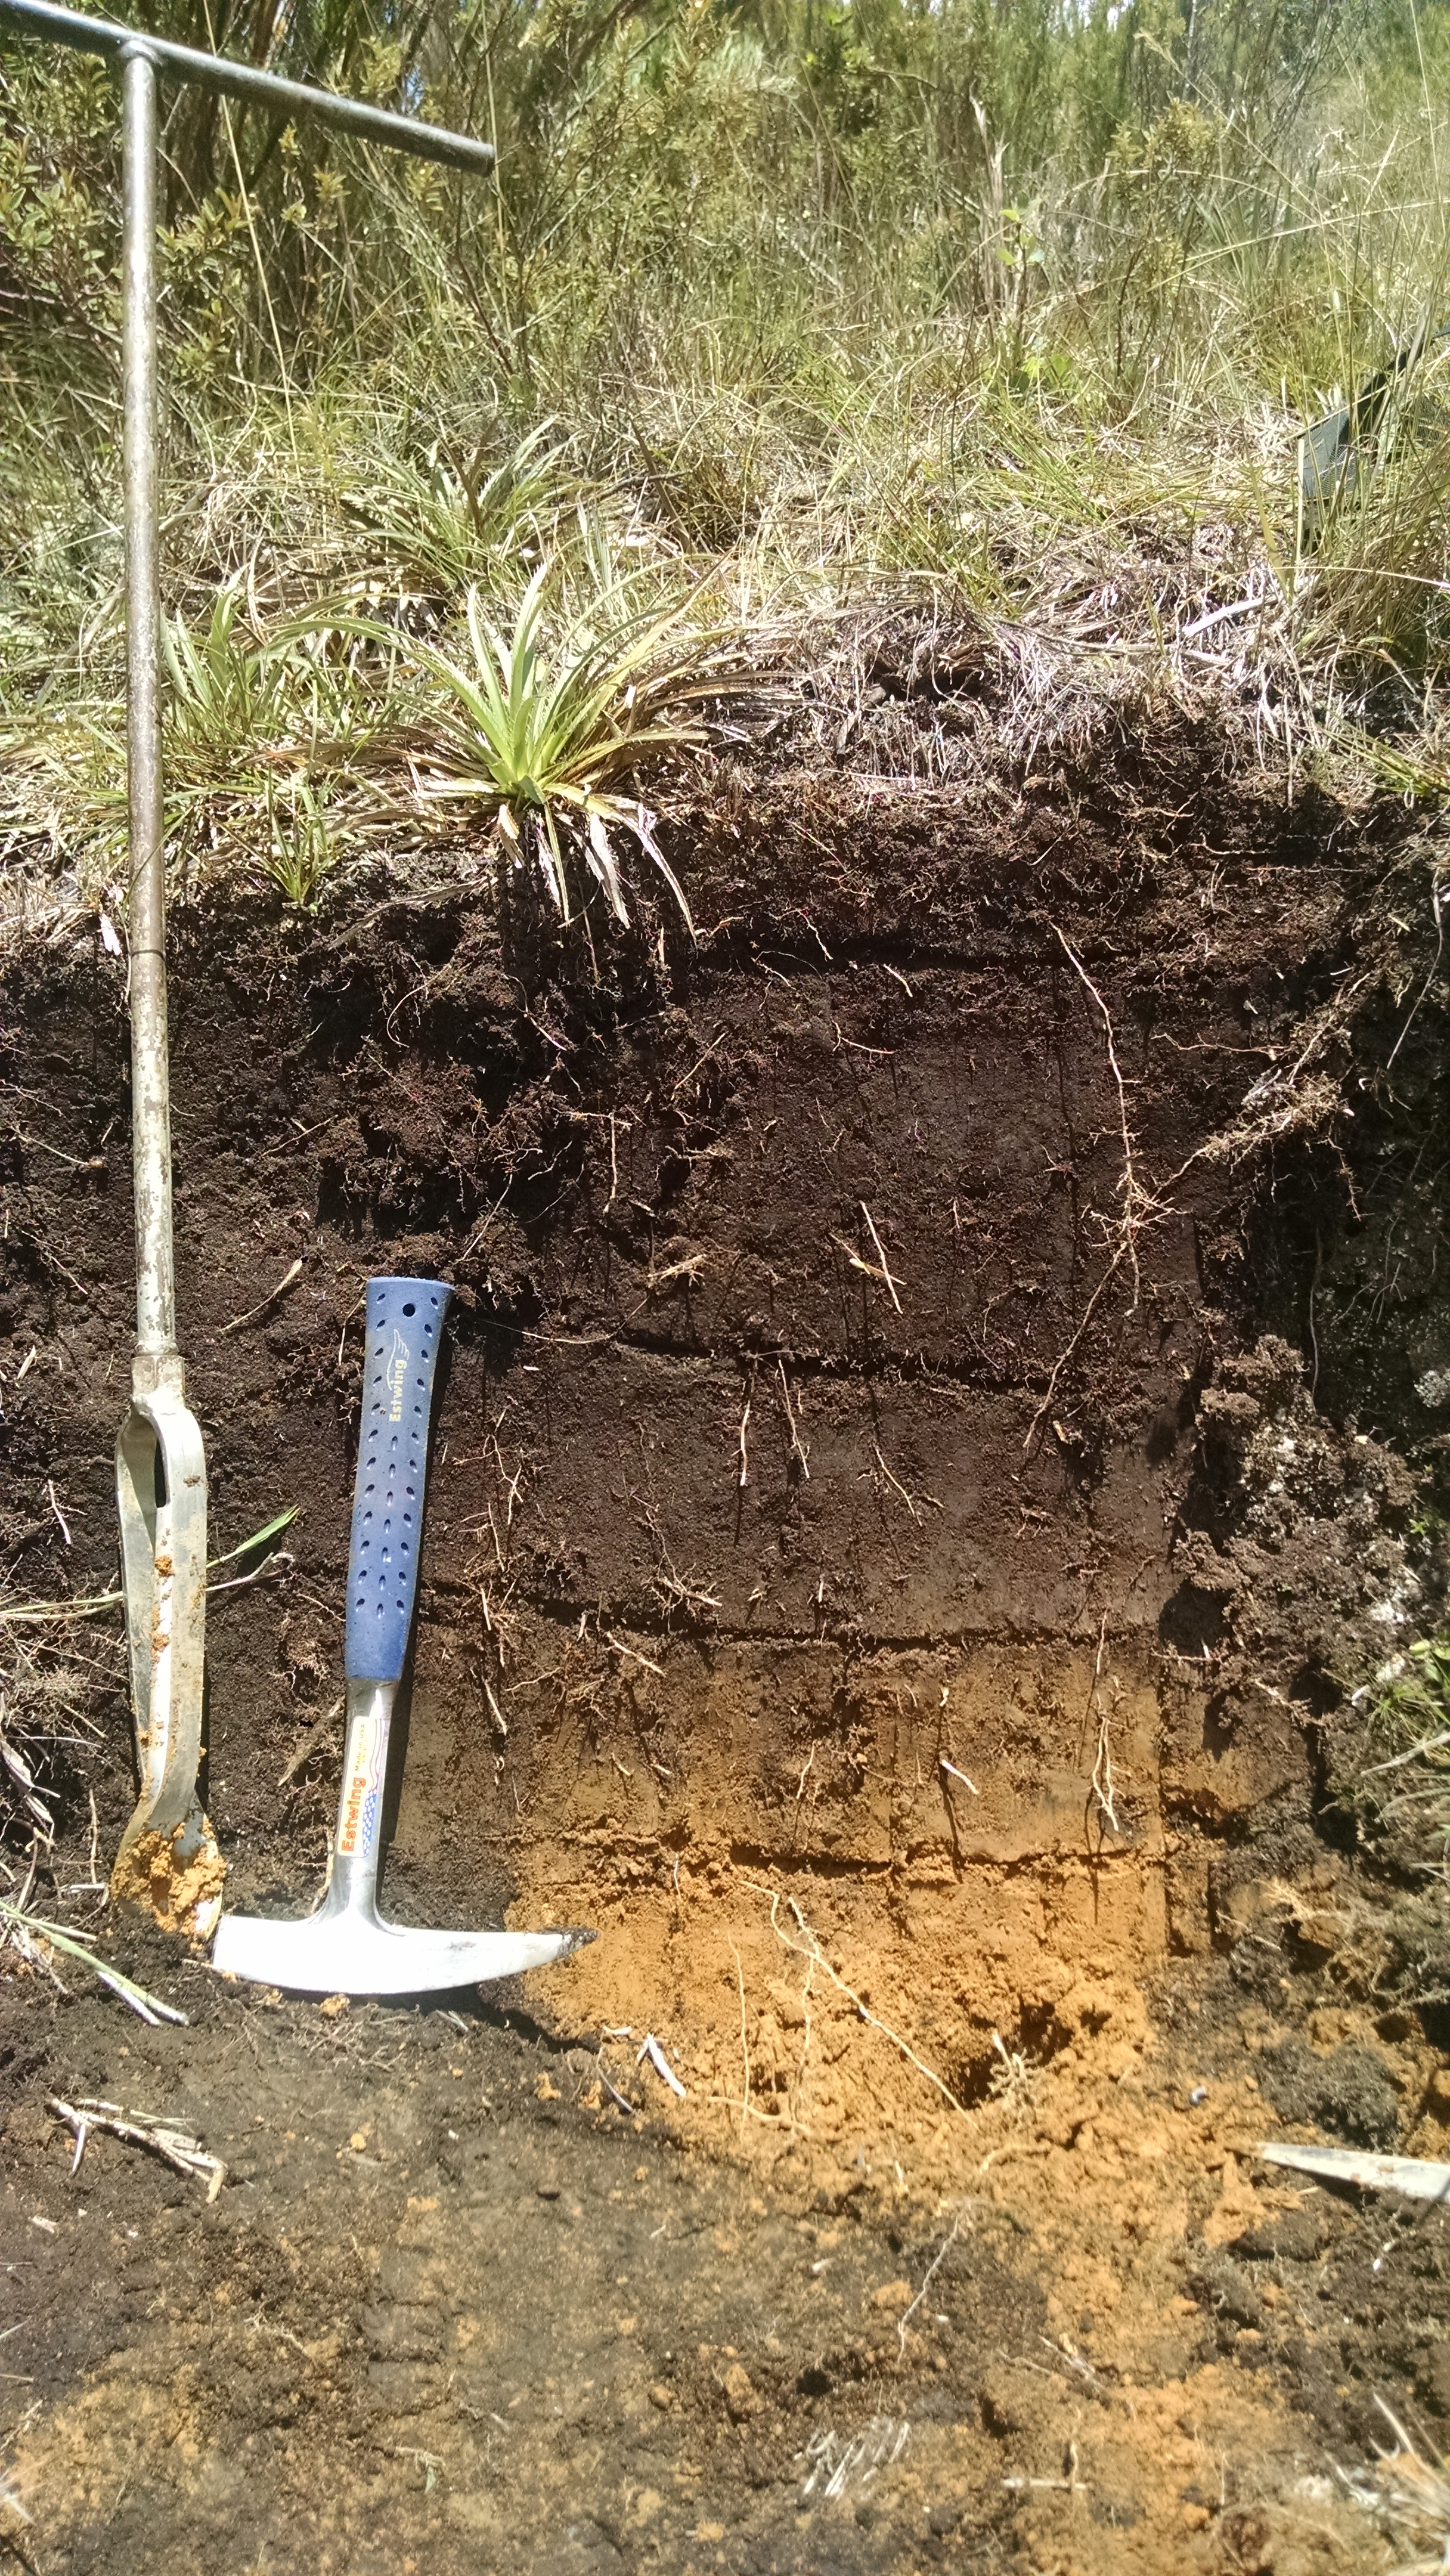
\includegraphics[width=5cm]{figures/soil.jpg} % leia abaixo
	\caption{Perfil de solo.}
	\label{fig1}
\end{figure}


\end{document}




















